\chapter{Materiales\label{ch:materiales}}
En este último capítulo, vamos a ver como dar color y texturas a los elementos de nuestra escena. Identificaremos cada elemento asignando un entero positivo \(id \in \mathbb{N}\) que será devuelto junto con la distancia a este objeto, es decir, vamos a devolver un \textit{vec2} cuya componente \enquote{x} será la distancia y cuya componente \enquote{y}, el identificador \(id\). Asignaremos la constante \(id=-1\) cuando no se ha trazado ningún objeto. Primero, vamos a modificar el \textit{Marcher} para que este pueda devolver ambos valores:

\begin{lstlisting}
// Devolvemos dos elementos, distancia e id.
vec2 SphereMarching(vec3 ojo, vec3 direccion){
    float distancia = 0.0;
    // Realizamos PASOS iteraciones de marching.
    for(int i = 0; i < PASOS; ++i){
        vec3 p = ojo + direccion * distancia;
        // La escena devuelve el radio de la bola y el id del elemento
        vec2 info = escena_sdf(p);
        // Factor para la sobreestimación.
        info.x *= 1.0;
        // info.x contiene la distancia
        if(abs(info.x) < EPSILON){
            // info.y contiene el id de un elemento de la escena.
            // Devolvemos la distancia acumulada (o distancia del ojo a la superficie) y el id.
            return vec2(distancia, info.y);
        }
        // incrementamos la distancia
        distancia += info.x;
        if(distancia >= MAXIMO) break;
    }
    // Devolvemos un id desconocido.
    return vec2(MAXIMO, -1);
}
\end{lstlisting}

El vector devuelto con nombre \textit{info}, toma los valores directamente de la escena, por lo que vamos a modificar el esquema de nuestra función \enquote{\textit{escena\_sdf}}, este ahora devolverá la distancia más cercana a un objeto y su identificador. El esquema será el siguiente:

\begin{lstlisting}
vec2 escena_sdf(vec3 p){
    // Identificador inicial y la distancia máxima.
    float id = -1.0;
    float min_dist = MAXIMO;
    
    // El esquema es el siguiente para cada figura de nuestra escena.
    // 1.Creamos nuestra primera figura.
    float sdf_0 = ....;
    // 2.Comprobamos que esta figura es la más cercana encontrada hasta el momento.
    if(sdf_0 < min_dist){
        // 2.1 En caso afirmativo, actualizamos los valores.
        // Asignamos el id de esta figura.
        id = 0.;
        // Actualizamos la distancia mínima como la distancia a esa figura.
        min_dist = sdf_0;
    }
    
    // Repetimos este esquema para cada elemento de la escena,
    float sdf_1 = ...;
    if(sdf_1 < min_dist){
        id = 1.;
        min_dist = sdf_1;
    }
    ...
    // Finalmente, devolvemos la distancia mínima y el objeto que la devuelve.
    return vec2(min_dist, id);
}
\end{lstlisting}

Al devolver ahora dos componentes, debemos modificar todas las funciones que hacían uso de esta función, donde encontramos \enquote{Normal} y \enquote{ModeloIluminacion}. Utilizamos el identificador devuelto para asignar un material, en código, recibe el nombre de \enquote{obtenerMaterial}. El material será multiplicado por la intensidad.
\[ \text{color}_{rgb}(id) = \text{obtenerMaterial}(id) \cdot I_{Phong} \]
Pongamos como ejemplo: una sección de un toro y una esfera, aplicando el esquema de código utilizado antes:

\begin{lstlisting}
vec2 escena_sdf(vec3 p){
    // ID inicial y distancia máxima.
    float id = -1.0;
    float min_dist = MAXIMO;
    // Toro rotado ri = 0.3 y r = 0.05. seccionado por un plano n=-z.
    float sdf_0 = max(
        SDFToro(rotYZ(p, PI / 4.), .3, .05),
        SDFPlano(p, vec3(0., 0., -1.))
    );
    // Comprobamos que sea la mas cercana.
    if(sdf_0 < min_dist){
        // Identificador del toro
        id = 0.;
        min_dist = sdf_0;
    }
    // Esfera de radio 0.2
    float sdf_1 = SDFEsfera(p, 0.2);
    // Comprobamos que sea la mas cercana.
    if(sdf_1 < min_dist){
        // Identificador de la esfera.
        id = 1.;
        min_dist = sdf_1;
    }
    // (distancia mínima, id)
    return vec2(min_dist, id);
}
\end{lstlisting}

\begin{figure}[H]
  \centering
  \captionsetup{justification=centering}%,margin=2cm
  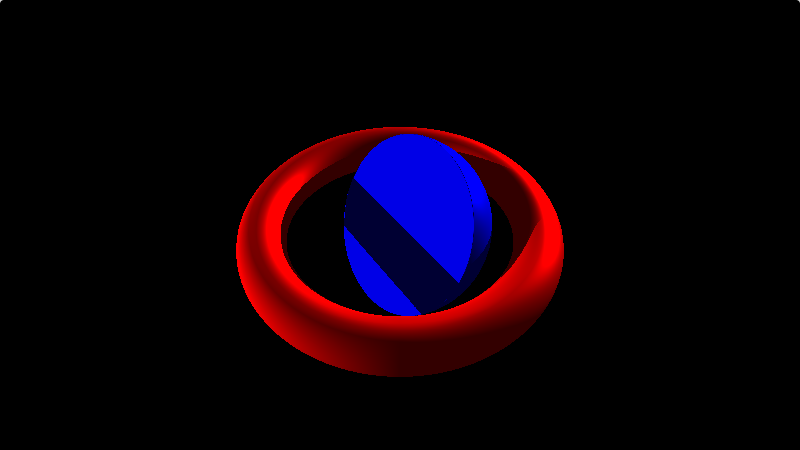
\includegraphics[width=1.0\textwidth]{secciones/imagenes/material/materiales.png}
  \caption{Materiales asignados a las distintas figuras.}
  \label{fig:material}
\end{figure}

Enlace del ejemplo:\url{https://www.shadertoy.com/view/wlBBRR}

En el ejemplo anterior, \textit{obtenerMaterial}, hace uso únicamente del identificador para devolver el color deseado:

\begin{lstlisting}
// Devuelve el color del material en el punto p
vec4 obtenerMaterial(vec3 p, float id){
    // Identificador del toro seccionado
    if(id == 0.){
        return vec4(1., 0., 0., 1.);
    }else if(id == 1.0){
        return vec4(0., 0., 1., 1.);
    }
}
\end{lstlisting}

Podemos utilizar el punto \(\Vec{p}\) para calcular la proyección hacia el sistema de coordenadas de alguna textura \cite{projections}. que accederemos utilizando el operador \enquote{texture} de \textit{GLSL}. Utilizaremos la textura creada en el ejemplo, \ref{fig:homotopies} y calcularemos las coordenadas de textura de la esfera, utilizando la proyección cilíndrica, ibíd. \enquote{Parametrization for two dimensional textures - Parametrization of implicit surfaces}.
\[\begin{pmatrix}
    u&
    v
\end{pmatrix}=  0.5\cdot
\begin{pmatrix}
    \dfrac{\arctan\left(\dfrac{\Vec{p}_x}{\Vec{p}_z}\right)}{\pi}+1&
    \Vec{p}_y + 1
\end{pmatrix}
\]

\begin{lstlisting}
// Devuelve el material en el punto p
vec4 obtenerMaterial(vec3 p, float id){
    // Identificador del toro seccionado
    if(id == 0.){
        return vec4(1., 0., 0., 1.);
    }else if(id == 1.0){
    	vec3 n = normalize(p);
        vec2 uv = 0.5 * vec2(
            atan(n.x, n.z) / PI + 1,
            n.y + 1
        );
        // Ejemplo : TFG 0-1 Homotopía
        vec4 text0 = texture(iChannel0,uv);
        vec4 text1 = texture(iChannel1,uv);
        float mascara = min(texture(iChannel2, uv*.25).r*2., 1.);
        vec3 homotopia = mix(text0.rgb, text1.rgb, h(mascara));
        // Devolvemos la textura
        return vec4(homotopia, 1.);
    }
}
\end{lstlisting}

El resultado:

\begin{figure}[H]
  \centering
  \captionsetup{justification=centering}%,margin=2cm
  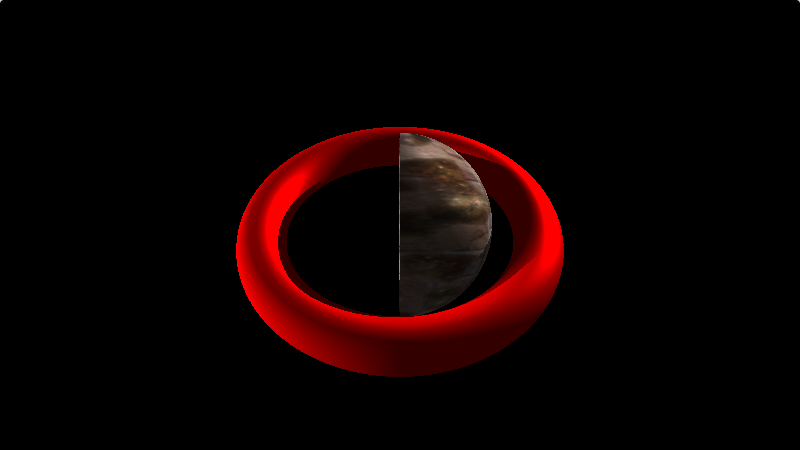
\includegraphics[width=1.0\textwidth]{secciones/imagenes/material/textura.png}
  \caption{Textura asignada a la semiesfera}
  \label{fig:texture}
\end{figure}

Enlace del ejemplo:\url{https://www.shadertoy.com/view/ttSBWD}